\section{Halton采样器}\label{sec:Halton采样器}
\begin{remark}
    本节含有高级内容,第一次阅读时可以跳过。
\end{remark}

\refvar{StratifiedSampler}{}的根本目标是生成
分布良好但不均匀的样本点集,使得不存在两个靠得太近的样本点且没有不含样本的过大样本空间区域。
如\reffig{7.18}{}所示,扰动的模式比随机模式做得更好,
不过当相邻层中的样本恰好靠近它们两层的公共边界时其质量可能受影响。

本节介绍\refvar{HaltonSampler}{},它基于直接生成低偏差点集的算法。不像\linebreak
\refvar{StratifiedSampler}{}生成的点集那样,
\refvar{HaltonSampler}{}不仅生成保证不会靠得太近抱团的点,
还生成能同时在样本向量所有维度上都分布良好的点——
而不是像\refvar{StratifiedSampler}{}那样每次只能在一两个维度上做到。

\subsection{Hammersley和Halton序列}\label{sub:Hammersley和Halton序列}
Halton和Hammersley序列是两种紧密相关的低偏差点集。
两者都基于称为\keyindex{倒根}{radical inverse}{}的构造法,
它基于正整数值$a$可以用下式唯一确定的数字序列$d_m(a)\ldots d_2(a)d_1(a)$
表示为$b$进制\sidenote{译者注:这里$b$是大于1的正整数,称为基(数)(base)。}的事实:
\begin{align}
    \label{eq:7.6}
    a=\sum\limits_{i=1}^m{d_i(a)b^{i-1}}\, ,
\end{align}
其中所有数字$d_i(a)$介于0到$b-1$之间。

$b$进制的倒根函数$\varPhi_b$通过将这些数字关于小数点翻转
把非负整数$a$转化为$[0,1)$的小数值:
\begin{align}
    \label{eq:7.7}
    \varPhi_b(a)=0.d_1(a)d_2(a)\ldots d_m(a)\, .
\end{align}
因此,数字$d_i(a)$对倒根的贡献为$\displaystyle\frac{d_i(a)}{b^i}$.

最简单的低偏差序列之一是van der Corput序列
\sidenote{译者注:得名自20世纪荷兰数学家Johannes Gaultherus van der Corput。},
它是由2进制倒根函数给出的1D序列:
\begin{align*}
    x_a=\varPhi_2(a)\, .
\end{align*}

\reftab{7.3}展示了van der Corput序列的前几个值。
注意它怎样递归地将1D直线上的区间对半划分,生成位于每个区间中心的的样本点。
\begin{table}[htbp]
    \centering
    \begin{tabular}{crl}
        \toprule
        $a$      & \textbf{2进制} & $\varPhi_2(a)$      \\
        \midrule
        0        & 0              & $0$                 \\
        1        & 1              & $0.1=\frac{1}{2}$   \\
        2        & 10             & $0.01=\frac{1}{4}$  \\
        3        & 11             & $0.11=\frac{3}{4}$  \\
        4        & 100            & $0.001=\frac{1}{8}$ \\
        5        & 101            & $0.101=\frac{5}{8}$ \\
        $\vdots$ &                &                     \\
        \bottomrule
    \end{tabular}
    \caption{以2进制计算的前几个非负整数的倒根$\varPhi_2(a)$.
        注意$\varPhi_2(a)$的后续值是怎样避开$\varPhi_2(a)$先前的任何值的。
        随着生成该序列越来越多的值,样本必然与之前的样本更加接近,然而仍保证了最小距离足够好。}
    \label{tab:7.3}
\end{table}

该序列的偏差为\sidenote{译者注:这里的大$O$项表明了该偏差的变化趋势。
    事实上它是有界的,相应证明非常复杂,读者可参见\citet{LARCHER2016546}整理的有关结论。}
\begin{align*}
    D^*_N(P)=O\left(\frac{\log N}{N}\right)\, ,
\end{align*}
它与$n$维无限序列取到的最优偏差相匹配,
\begin{align*}
    D^*_N(P)=O\left(\frac{(\log N)^n}{N}\right)\, .
\end{align*}

为了生成$n$维Halton序列,我们使用$b$进制倒根,且模式的每个维度用不同的基。
所用的基必须两两互质,所以自然的选择是使用
前$n$个\keyindex{质数}{prime number}{}$(p_1,\ldots,p_n)$:
\begin{align*}
    x_a=(\varPhi_2(a),\varPhi_3(a),\varPhi_5(a),\ldots,\varPhi_{p_n}(a))\, .
\end{align*}

Halton序列最有用的性质之一是即使不能提前知道所需的样本总量也能用它;
该序列的所有前缀\sidenote{译者注:即序列开头的部分。}都分布良好,
所以向该序列添加额外样本也可保持低偏差(然而对于指数$k_i$,
当样本总数为基的幂之积$\prod(p_i)^{k_i}$时其分布最好)。

$n$维Halton序列的偏差为
\begin{align*}
    D^*_N(x_a)=O\left(\frac{(\log N)^n}{N}\right)\, ,
\end{align*}
它是渐进最优的。

如果固定样本数目$N$,则可以用偏差还低点的Hammersley点集。
Hammersley点集定义为
\begin{align*}
    x_a=\left(\frac{a}{N},\varPhi_{b_1}(a),\varPhi_{b_2}(a),\ldots,\varPhi_{b_n}(a),\right)\, ,
\end{align*}
其中$N$是要取用的样本总数,像之前那样所有基$b_i$都互质。
\reffig{7.25.1}展示了2D Halton序列前216个点的图示。
\reffig{7.25.2}展示了Hammersley序列的前256个点。
\begin{figure}[htbp]
    \centering
    \subfloat[]{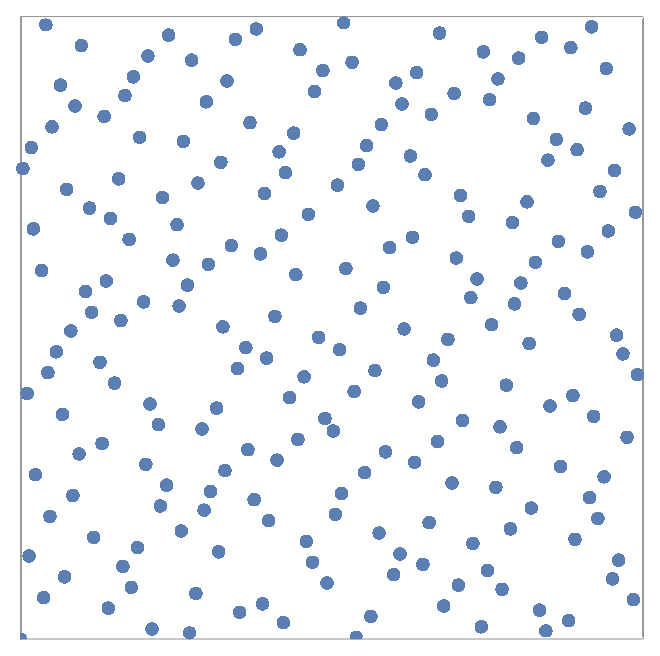
\includegraphics[width=0.49\linewidth]{chap07/halton-points.eps}\label{fig:7.25.1}}\,
    \subfloat[]{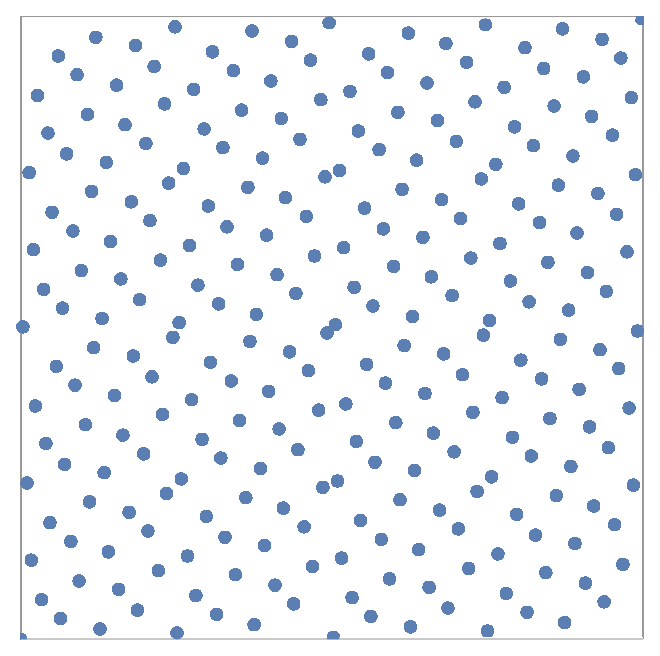
\includegraphics[width=0.49\linewidth]{chap07/hammersley-points.eps}\label{fig:7.25.2}}
    \caption{两种2D低偏差序列前面的点。(a)Halton(216个点),(b)Hammersley(256个点)。}
    \label{fig:7.25}
\end{figure}

函数\refvar{RadicalInverse}{()}用第{\ttfamily baseIndex}个质数
作为基为给定数字{\ttfamily a}计算倒根。
该函数用庞大的{\ttfamily switch}语句实现,其中{\ttfamily baseIndex}被映射到
合适的质数然后由单独的模板函数\refvar{RadicalInverseSpecialized}{()}实际计算该倒根
(稍后将解释使用少见的基于{\ttfamily switch}的结构的原因)。
\begin{lstlisting}
`\initcode{Low Discrepancy Function Definitions}{=}\initnext{LowDiscrepancyFunctionDefinitions}`
`\refvar{Float}{}` `\initvar{RadicalInverse}{}`(int baseIndex, uint64_t a) {
    switch (baseIndex) {
        case 0:
            `\refcode{Compute base-2 radical inverse}{}`
        case 1: return `\refvar{RadicalInverseSpecialized}{}`<3>(a);
        case 2: return `\refvar{RadicalInverseSpecialized}{}`<5>(a);
        case 3: return `\refvar{RadicalInverseSpecialized}{}`<7>(a);
        `\refcode{Remainder of cases for RadicalInverse()}{}`
    }
}
\end{lstlisting}

对于2进制倒根,我们可以利用数字计算机中的数字已经表示为2进制的事实
来更高效地计算倒根。对于一个64位值$a$,按\refeq{7.6}我们有
\begin{align*}
    a=\sum\limits_{i=1}^{64}{d_i(a)2^{i-1}}\, .
\end{align*}
首先考虑翻转$a$数位的结果,仍将其视作整数值,得到
\begin{align*}
    \sum\limits_{i=1}^{64}{d_i(a)2^{64-i}}\, .
\end{align*}
如果我们再用该值除以$2^{64}$,我们有
\begin{align*}
    \sum\limits_{i=1}^{64}{d_i(a)2^{-i}}\, ,
\end{align*}
它就是$\varPhi_2(a)$.因此,2进制倒根可高效地用数位翻转以及2的幂除法算得。

整数量的数位可以用一系列逻辑位运算高效翻转。
翻转32位整数数位的函数\refvar{ReverseBits32}{()}的第一行
交换了该值的低16位和高16位。下一行同时交换其结果的前8位与第二组8位、第三组8位与第四组。
该过程持续到交换相邻数位的最后一行。为了理解该代码,写出各个十六进制常数的二进制值很有帮助。
例如,{\ttfamily 0xff00ff00}的二进制是{\ttfamily 11111111000000001111111100000000};
很容易看到与该值进行按位或屏蔽了第一、三组8位数量。
\begin{lstlisting}
`\initcode{Low Discrepancy Inline Functions}{=}\initnext{LowDiscrepancyInlineFunctions}`
inline uint32_t `\initvar{ReverseBits32}{}`(uint32_t n) {
    n = (n << 16) | (n >> 16);
    n = ((n & 0x00ff00ff) << 8) | ((n & 0xff00ff00) >> 8);
    n = ((n & 0x0f0f0f0f) << 4) | ((n & 0xf0f0f0f0) >> 4);
    n = ((n & 0x33333333) << 2) | ((n & 0xcccccccc) >> 2);
    n = ((n & 0x55555555) << 1) | ((n & 0xaaaaaaaa) >> 1);
    return n;
}
\end{lstlisting}

然后通过单独翻转两个32位分量再互换它们可以翻转64位值的数位。
\begin{lstlisting}
`\refcode{Low Discrepancy Inline Functions}{+=}\lastnext{LowDiscrepancyInlineFunctions}`
inline uint64_t `\initvar{ReverseBits64}{}`(uint64_t n) {
    uint64_t n0 = `\refvar{ReverseBits32}{}`((uint32_t)n);
    uint64_t n1 = `\refvar{ReverseBits32}{}`((uint32_t)(n >> 32));
    return (n0 << 32) | n1;
}
\end{lstlisting}

然后为了计算2进制倒根,我们翻转数位并乘以$\displaystyle\frac{1}{2^{64}}$,
其中十六进制浮点常数{\ttfamily 0x1p-64}用于值$2^{-64}$.
如\refsub{浮点算术}解释的,通过相应的幂2乘法实现幂2除法
会给出以IEEE浮点数表示的相同结果(且浮点数乘法通常比浮点数除法更高效)。
\begin{lstlisting}
`\initcode{Compute base-2 radical inverse}{=}`
return `\refvar{ReverseBits64}{}`(a) * 0x1p-64;
\end{lstlisting}

对于其他基,模板函数\refvar{RadicalInverseSpecialized}{()}计算倒根
是通过计算起始于$d_1$的数字$d_i$并计算一系列$v_i$,
其中$v_1=d_1$,$v_2=bd_1+d_2$,使得
\begin{align*}
    v_n=b^{n-1}d_1+b^{n-2}d_2+\cdots+d_n\, .
\end{align*}
(例如,十进制中它会把值1234转化为4321.)
该值可完全用整数算法求得,不会积累任何舍入误差。

然后倒根的最终值通过转化为浮点并乘以$\displaystyle\frac{1}{b^n}$求得,
其中$n$是该值的位数,由此得到\refeq{7.7}中的值。
该乘法项是在处理数字时在{\ttfamily invBaseN}中构建的。
\begin{lstlisting}
`\initcode{Low Discrepancy Static Functions}{=}\initnext{LowDiscrepancyStaticFunctions}`
template <int base>
static `\refvar{Float}{}` `\initvar{RadicalInverseSpecialized}{}`(uint64_t a) {
    const `\refvar{Float}{}` invBase = (`\refvar{Float}{}`)1 / (`\refvar{Float}{}`)base;
    uint64_t reversedDigits = 0;
    `\refvar{Float}{}` invBaseN = 1;
    while (a) {
        uint64_t next  = a / base;
        uint64_t digit = a - next * base;
        reversedDigits = reversedDigits * base + digit;
        invBaseN *= invBase;
        a = next;
    }
    return std::min(reversedDigits * invBaseN, `\refvar{OneMinusEpsilon}{}`);
}
\end{lstlisting}

一个自然要问的问题是为什么这里要用对基数做参数化的模板函数
(而不是说调用一个把基数作为参数接收的常规函数,避免为每个基生成单独的代码路径)。
动机是在现代CPU上整数除法非常地慢,利用编译时常数除法的方法则能高效得多。

例如,32位值除以3的整数除法可以通过用该值乘以2863311531得到64位中间值
然后将结果右移33位算得;这俩都是非常高效的运算。
(64位值除以3可以用类似方法,但这个神奇常数大得多;
见\citet{10.5555/2462741}\sidenote{译者注:此处引用改为了新版。}了解关于该技术的更多内容。)
因此这里用模板函数允许编译器意识到在{\ttfamily while}循环中计算{\ttfamily next}值的除法时
实际上是除以常数并给它应用该优化的机会。在2015年代笔记本上用了该优化的代码比
基于整数除法指令的实现运行起来快至5.9倍。

另一个优化是我们避免计算翻转数字与倒数基之积的实时总和;
相反,该乘法会一直推迟到结尾直到循环终止。
这里的主要问题是当前处理器的浮点和整数单元是完全互相独立运算的。
在一个紧密循环里的浮点计算中引用一个整数变量会引入管道暂停
\sidenote{译者注:原文pipeline bubble。},
它与转化这些值并从一个单元移动到另一个单元所需的时间相关。

能计算倒根函数的逆会很有用;函数\refvar{InverseRadicalInverse}{()}接收
某进制翻转过的整数数字,即对应于模板函数\refvar{RadicalInverseSpecialized}{()}中
为了转化为$[0,1)$中的浮点值而乘以因子$\displaystyle\frac{1}{b^n}$之前的{\ttfamily reversedDigits}。
注意为了能正确地计算逆,必须知道原始值中的数字总数:
例如倒根算法中在只含整数的部分之后,1234和123400都能转化为4321;
尾部零变为前导零并丢失了。
\begin{lstlisting}
`\refcode{Low Discrepancy Inline Functions}{+=}\lastnext{LowDiscrepancyInlineFunctions}`
template <int base> inline uint64_t
`\initvar{InverseRadicalInverse}{}`(uint64_t inverse, int nDigits) {
    uint64_t index = 0;
    for (int i = 0; i < nDigits; ++i) {
        uint64_t digit = inverse % base;
        inverse /= base;
        index = index * base + digit;
    }
    return index;
}
\end{lstlisting}

Hammersley和Halton序列的缺点是随着基$b$的增加,样本值会展现出惊人的规律模式。
该问题可以用\keyindex{置乱}{scrambled}{}Halton和Hammersley序列解决,
其计算倒根时对数字施加了重排。
\begin{align}
    \label{eq:7.8}
    \varPsi_b(a)=0.p(d_1(a))p(d_2(a))\ldots p(d_m(a))\, ,
\end{align}
其中$p$是数字$(0,1,\ldots,b-1)$的重排。
注意每个数字用的重排是一样的,在给定基$b$下生成所有样本点用的重排也一样。
\reffig{7.26}展示了对Halton序列置乱后的效果。
\begin{figure}[htbp]
    \centering
    \subfloat[]{
\includegraphics[width=0.45\linewidth]{chap07/halton2931.eps}\label{fig:7.26.1}}\,
    \subfloat[]{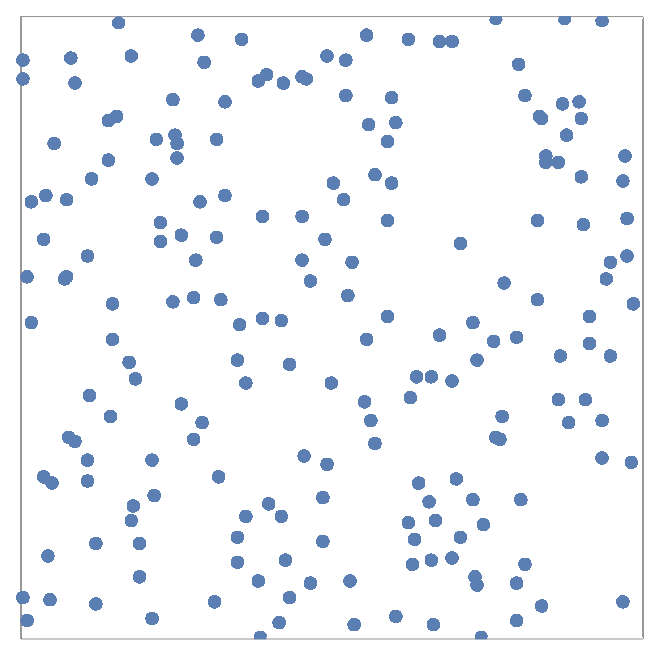
\includegraphics[width=0.45\linewidth]{chap07/halton2931-permuted.eps}\label{fig:7.26.2}}
    \caption{Halton样本值是否有置乱的图示。(a)在样本向量的高维中,
        样本值的投影开始表现出规律结构。这里展示了来自维度$(\varPhi_{29}(a),\varPhi_{31}(a))$的点。
        (b)置乱序列即\refeq{7.8}通过随机重排样本索引的数字打破了该结构。}
    \label{fig:7.26}
\end{figure}

尽管专门构造的重排能给出稍微更好的结构,但接下来我们将用随机重排;
见“扩展阅读”一节了解更多细节。

函数\refvar{ComputeRadicalInversePermutations}{()}计算这些随机重排表。
它为所有重排初始化单个连续数组,其前两个值是$b=2$时整数零和一的重排,
接下来三个值是$b=3$时0、1、2的重排,后续质数基以此类推。
在进入下面的{\ttfamily for}循环时,{\ttfamily p}指向重排数组的起点来为当前的质数基做初始化。
\begin{lstlisting}
`\refcode{Low Discrepancy Function Definitions}{+=}\lastnext{LowDiscrepancyFunctionDefinitions}`
std::vector<uint16_t> `\initvar{ComputeRadicalInversePermutations}{}`(`\refvar{RNG}{}` &rng) {
    std::vector<uint16_t> perms;
    `\refcode{Allocate space in perms for radical inverse permutations}{}`
    uint16_t *p = &perms[0];
    for (int i = 0; i < `\refvar{PrimeTableSize}{}`; ++i) {
        `\refcode{Generate random permutation for ith prime base}{}`
        p += `\refvar{Primes}{}`[i];
    }
    return perms;
}
\end{lstlisting}

重排数组的总大小由直到预先计算的质数表末尾的质数之和给出。
\begin{lstlisting}
`\initcode{Allocate space in perms for radical inverse permutations}{=}`
int permArraySize = 0;
for (int i = 0; i < `\refvar{PrimeTableSize}{}`; ++i)
    permArraySize += `\refvar{Primes}{}`[i];
perms.resize(permArraySize);
\end{lstlisting}
\begin{lstlisting}
`\initcode{Low Discrepancy Declarations}{=}\initnext{LowDiscrepancyDeclarations}`
static constexpr int `\initvar{PrimeTableSize}{}` = 1000;
extern const int `\initvar{Primes}{}`[`\refvar{PrimeTableSize}{}`];
\end{lstlisting}
\begin{lstlisting}
`\initcode{Low Discrepancy Data Definitions}{=}\initnext{LowDiscrepancyDataDefinitions}`
const int `\refvar{Primes}{}`[`\refvar{PrimeTableSize}{}`] = {
    2, 3, 5, 7, 11,
    `\refcode{Subsequent prime numbers}{}`
};
\end{lstlisting}

生成每次重排很简单:我们只需初始化{\ttfamily p}使之指向
对应当前质数长度的同一重排然后随机打乱它的值。
\begin{lstlisting}
`\initcode{Generate random permutation for ith prime base}{=}`
for (int j = 0; j < `\refvar{Primes}{}`[i]; ++j)
    p[j] = j;
`\refvar{Shuffle}{}`(p, `\refvar{Primes}{}`[i], 1, rng);
\end{lstlisting}

函数\refvar{ScrambledRadicalInverse}{()}本质上和\refvar{RadicalInverse}{()}一样,
除了它是通过重排表为给定基数放入每个数字的。
见\refvar{RadicalInverse}{()}之后的习题\ref{sub:7.11.3}了解关于2进制情况下的更高效实现的讨论。
\begin{lstlisting}
`\refcode{Low Discrepancy Function Definitions}{+=}\lastcode{LowDiscrepancyFunctionDefinitions}`
`\refvar{Float}{}` `\initvar{ScrambledRadicalInverse}{}`(int baseIndex, uint64_t a,
        const uint16_t *perm) {
    switch (baseIndex) {
        case 0: return `\refvar{ScrambledRadicalInverseSpecialized}{}`<2>(perm, a);
        case 1: return `\refvar{ScrambledRadicalInverseSpecialized}{}`<3>(perm, a);
        case 2: return `\refvar{ScrambledRadicalInverseSpecialized}{}`<5>(perm, a);
        case 3: return `\refvar{ScrambledRadicalInverseSpecialized}{}`<7>(perm, a);
        `\refcode{Remainder of cases for ScrambledRadicalInverse()}{}`
    }
}
\end{lstlisting}

下面的实现也考虑了当{\ttfamily perm}将数字0映射为非零值时可能出现的特殊情况。
该情况下,一旦{\ttfamily a}到达0迭代就提前停止,
错误地漏掉了值{\ttfamily perm[0]}构成的无限长后继。
幸运的是,这是一个有简单解析解的几何级数,最后一行加上了其值
\sidenote{译者注:以$b=4$、{\ttfamily perm}数组为$[3,2,1,0]$、$a=9$时为例:
$a$以四进制表示为$21$,翻转得$12$,变为四进制浮点数为$0.12$,准确点说是$0.120000\ldots$.
按照重排表{\ttfamily perm}替换数字后应为$0.213333\ldots$.
但代码只处理到前两位即0.21,故应手动加上后面的$0.003333\ldots$.
一般地,应补充的$b$进制数字为$0.\underbrace{0\ldots0}_{m\text{个}0}p(0)p(0)p(0)\ldots$,
其中$m$为$a$的$b$进制位数,依据等比数列求和公式可得
其值是$\displaystyle\frac{b^{-1}p(0)}{1-b^{-1}}b^{-m}$.}。
\begin{lstlisting}
`\refcode{Low Discrepancy Static Functions}{+=}\lastcode{LowDiscrepancyStaticFunctions}`
template <int base>
static `\refvar{Float}{}` `\initvar{ScrambledRadicalInverseSpecialized}{}`(const uint16_t *perm,
        uint64_t a) {
    const `\refvar{Float}{}` invBase = (`\refvar{Float}{}`)1 / (`\refvar{Float}{}`)base;
    uint64_t reversedDigits = 0;
    `\refvar{Float}{}` invBaseN = 1;
    while (a) {
        uint64_t next  = a / base;
        uint64_t digit = a - next * base;
        reversedDigits = reversedDigits * base + perm[digit];
        invBaseN *= invBase;
        a = next;
    }
    return std::min(invBaseN * (reversedDigits +
                    invBase * perm[0] / (1 - invBase)), `\refvar{OneMinusEpsilon}{}`);
}
\end{lstlisting}

\subsection{Halton采样器实现}\label{sub:Halton采样器实现}
\refvar{HaltonSampler}{}用Halton序列生成样本向量。
不像\refvar{StratifiedSampler}{}那样,它是完全确定性的;
在其运算中它没有使用伪随机数。然而,如果没有充分采样好图像,
则Halton样本可能导致混叠。\reffig{7.27}比较了用基于Halton的采样器
和用上一节的分层采样器来采样棋盘纹理的结果。
注意前景中以及朝向地平线处沿边缘的令人难受的模式。
\begin{figure}[htbp]
    \centering
    \subfloat[1个扰动样本]{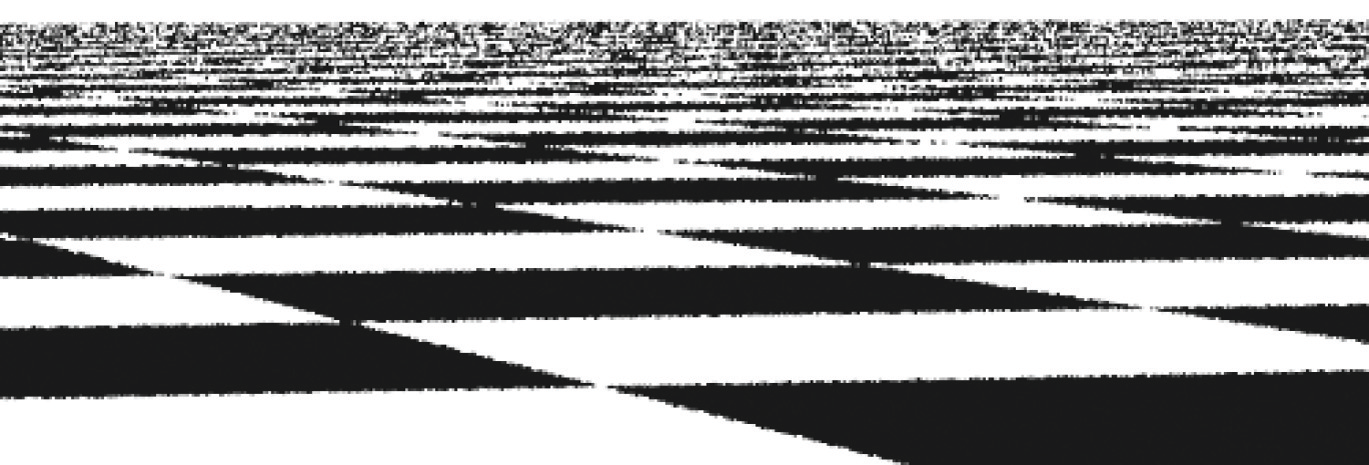
\includegraphics[width=\linewidth]{chap07/checkerboard-jitter-1spp.png}\label{fig:7.27.1}}\\
    \subfloat[1个Halton样本]{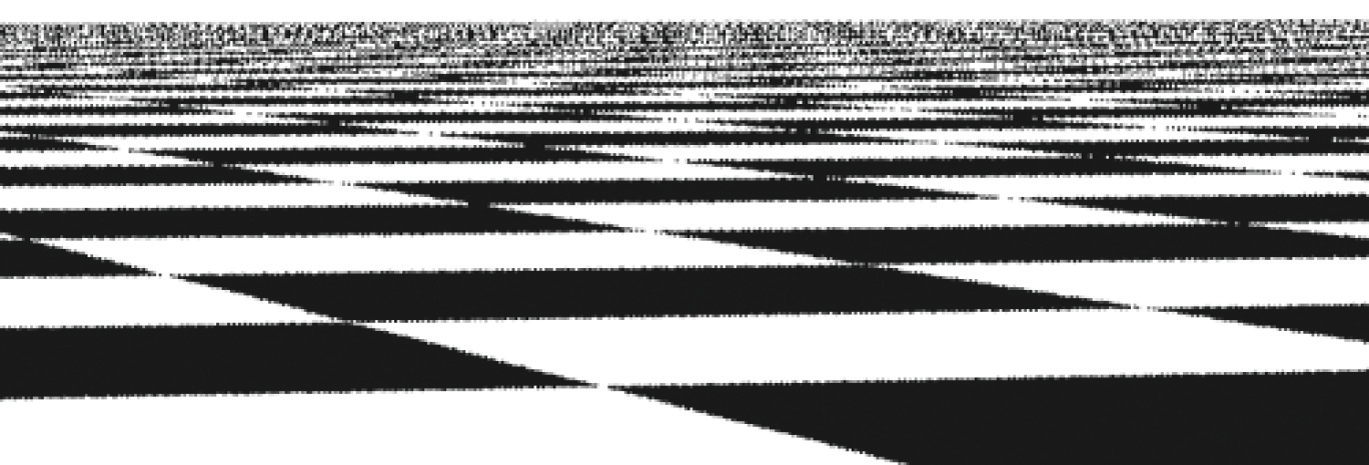
\includegraphics[width=\linewidth]{chap07/checkerboard-halton-1spp.png}\label{fig:7.27.2}}
    \caption{在图像平面上比较分层采样器和基于Halton点的低偏差采样器。
        (a)每个像素只有单个样本的扰动分层采样器与(b)每个像素只有单个样本的\refvar{HaltonSampler}{}采样器。
        注意尽管Halton模式比分层模式更能复现朝向地平线处的棋盘模式,
        但在低偏差模式中仍有干扰视觉注意力的规律性错误结构;
        它没有像扰动法那样把混叠转化为不那么讨厌的噪声。}
    \label{fig:7.27}
\end{figure}

\begin{lstlisting}
`\initcode{HaltonSampler Declarations}{=}`
class `\initvar{HaltonSampler}{}` : public `\refvar{GlobalSampler}{}` {
public:
    `\refcode{HaltonSampler Public Methods}{}`
private:
    `\refcode{HaltonSampler Private Data}{}`
    `\refcode{HaltonSampler Private Methods}{}`
};
\end{lstlisting}
\begin{lstlisting}
`\initcode{HaltonSampler Method Definitions}{=}\initnext{HaltonSamplerMethodDefinitions}`
`\refvar{HaltonSampler}{}`::`\refvar{HaltonSampler}{}`(int samplesPerPixel,
        const `\refvar{Bounds2i}{}` &sampleBounds)
    : `\refvar{GlobalSampler}{}`(samplesPerPixel) {
    `\refcode{Generate random digit permutations for Halton sampler}{}`
    `\refcode{Find radical inverse base scales and exponents that cover sampling area}{}`
    `\refcode{Compute stride in samples for visiting each pixel area}{}`
    `\refcode{Compute multiplicative inverses for baseScales}{}`
}
\end{lstlisting}
\begin{lstlisting}
`\initcode{HaltonSampler Public Methods}{=}`
`\refvar{HaltonSampler}{}`(int nsamp, const `\refvar{Bounds2i}{}` &sampleBounds);
int64_t `\refvar[HaltonSampler::GetIndexForSample]{GetIndexForSample}{}`(int64_t sampleNum) const;
`\refvar{Float}{}` `\refvar[HaltonSampler::SampleDimension]{SampleDimension}{}`(int64_t index, int dimension) const;
std::unique_ptr<`\refvar{Sampler}{}`> `\refvar{Clone}{}`(int seed);
\end{lstlisting}
\begin{lstlisting}
`\initcode{Compute multiplicative inverses for baseScales}{=}`
`\refvar{multInverse}{}`[0] = `\refvar{multiplicativeInverse}{}`(`\refvar{baseScales}{}`[1], `\refvar{baseScales}{}`[0]);
`\refvar{multInverse}{}`[1] = `\refvar{multiplicativeInverse}{}`(`\refvar{baseScales}{}`[0], `\refvar{baseScales}{}`[1]);
\end{lstlisting}

置乱倒根的重排表在所有\refvar{HaltonSampler}{}实例间
共享并在构造函数首次运行时算出。对pbrt的需求而言,该方法很好:
当前实现只是为不同图块使用不同采样器实例,而那时我们想总是使用相同的重排。
对于其他用途,对何时使用不同的重排有更强的控制是值得的。
\begin{lstlisting}
`\initcode{Generate random digit permutations for Halton sampler}{=}`
if (`\refvar{radicalInversePermutations}{}`.size() == 0) {
    `\refvar{RNG}{}` rng;
    `\refvar{radicalInversePermutations}{}` = `\refvar{ComputeRadicalInversePermutations}{}`(rng);
}
\end{lstlisting}
\begin{lstlisting}
`\initcode{HaltonSampler Private Data}{=}\initnext{HaltonSamplerPrivateData}`
static std::vector<uint16_t> `\initvar{radicalInversePermutations}{}`;
\end{lstlisting}

实用方法\refvar{PermutationForDimension}{()}为给定
维度返回指向重排数组起点的指针。
\begin{lstlisting}
`\initcode{HaltonSampler Private Methods}{=}`
const uint16_t *`\initvar{PermutationForDimension}{}`(int dim) const {
    if (dim >= `\refvar{PrimeTableSize}{}`)
        `\refvar{Severe}{}`("HaltonSampler can only sample %d dimensions.",
               `\refvar{PrimeTableSize}{}`);
    return &`\refvar{radicalInversePermutations}{}`[`\refvar{PrimeSums}{}`[dim]];
}
\end{lstlisting}

为了能为给定维度快速找到偏移量,拥有每个质数之前的所有质数之和是很有帮助的。
\begin{lstlisting}
`\refcode{Low Discrepancy Data Definitions}{+=}\lastcode{LowDiscrepancyDataDefinitions}`
const int `\initvar{PrimeSums}{}`[`\refvar{PrimeTableSize}{}`] = {
    0, 2, 5, 10, 17, 
    `\refcode{Subsequent prime sums}{}`
};
\end{lstlisting}

为了把来自$[0,1)^2$的样本前两维映射为像素坐标,
\refvar{HaltonSampler}{}在每个维度上求得比图像分辨率
和\refvar{kMaxResolution}{}中较小者更大的最小缩放因子$(2^j,3^k)$
(我们稍后将看到这一专门选出的缩放值是怎样让看出一个样本在哪个像素里变简单的)。
缩放之后,任何图像范围之外的样本都被简单忽略掉。

对于分辨率在一或两维上大于\refvar{kMaxResolution}{}的图像,
则在全图上重复一块Halton点。该分辨率限制帮助在算得的样本值中保持足够的浮点精度。
\begin{lstlisting}
`\initcode{Find radical inverse base scales and exponents that cover sampling area}{=}`
`\refvar{Vector2i}{}` res = sampleBounds.`\refvar{pMax}{}` - sampleBounds.`\refvar{pMin}{}`;
for (int i = 0; i < 2; ++i) {
    int base = (i == 0) ? 2 : 3;
    int scale = 1, exp = 0;
    while (scale < std::min(res[i], `\refvar{kMaxResolution}{}`)) {
        scale *= base;
        ++exp;
    }
    `\refvar{baseScales}{}`[i] = scale;
    `\refvar{baseExponents}{}`[i] = exp;
}
\end{lstlisting}

对于每个维度,\refvar{baseScales}{}存有缩放因子$2^j$或$3^k$,
且\refvar{baseExponents}{}存有指数$j$和$k$.
\begin{lstlisting}
`\refcode{HaltonSampler Private Data}{+=}\lastnext{HaltonSamplerPrivateData}`
`\refvar{Point2i}{}` `\initvar{baseScales}{}`, `\initvar{baseExponents}{}`;
\end{lstlisting}
\begin{lstlisting}
`\initcode{HaltonSampler Local Constants}{=}`
static constexpr int `\initvar{kMaxResolution}{}` = 128;
\end{lstlisting}

为了明白为什么\refvar{HaltonSampler}{}使用该方案来
将样本映射到像素坐标,考虑用$b$进制倒根因子$b^n$来缩放算出的值的影响。
如果$a$的数字表示为$b$进制的$d_i(a)$,则回想倒根为$b$进制的值$0.d_1(a)d_2(a)\ldots$.
例如,如果我们用$b^2$乘以该值,则我们有$d_1(a)d_2(a).d_3(a)\ldots$;
前两个数字被移到小数点左边,该值的小数部分从$d_3(a)$开始。

用$b^n$缩放的该运算构建了能够确定哪个样本索引位于哪个像素中的核心。
考虑上面例子中的前两个数字,我们可以看到缩放后的值的整数部分在0到$b^2-1$的范围内,
且随着$a$增加,在该范围内每过$b^2$个值,其$b$进制的最后两个数字就在某特定值上取得一次。

给定值$x$,$0\le x\le b^2-1$,我们可以求得首个整数部分为$x$的值$a$.
根据定义,$b$进制的$x$数字为$d_2(x)d_1(x)$.
因此,如果$d_1(a)=d_2(x)$且$d_2(a)=d_1(x)$,
则$a$的倒根被缩放后的值会有等于$x$的整数部分。

因为\refvar{HaltonSampler}{}中为像素样本用的基$b=2$和$b=3$是互质的,
所以它满足如果样本值由某个$(2^j,3^k)$缩放,则在
范围$(0,0)\rightarrow(2^j-1,3^k-1)$内的任意特定像素
每过$2^j3^k$个样本就会访问一次。该乘积存于\refvar{sampleStride}{}中。
\begin{lstlisting}
`\initcode{Compute stride in samples for visiting each pixel area}{=}`
`\refvar{sampleStride}{}` = `\refvar{baseScales}{}`[0] * `\refvar{baseScales}{}`[1];
\end{lstlisting}
\begin{lstlisting}
`\refcode{HaltonSampler Private Data}{+=}\lastnext{HaltonSamplerPrivateData}`
int `\initvar{sampleStride}{}`;
\end{lstlisting}
\begin{lstlisting}
`\refcode{HaltonSampler Private Data}{+=}\lastnext{HaltonSamplerPrivateData}`
int `\initvar{multInverse}{}`[2];
\end{lstlisting}

位于\refvar{currentPixel}{}内的首个Halton样本的样本索引存于\refvar{offsetForCurrentPixel}{}
中。在为当前像素中的首个样本算出该偏移量后,该像素中的后续样本
可在Halton序列中增量为\refvar{sampleStride}{}的样本处找到
\sidenote{译者注:指索引每增加\refvar{sampleStride}{}就出现一次该像素的样本。}。
\begin{lstlisting}
`\refcode{HaltonSampler Method Definitions}{+=}\lastnext{HaltonSamplerMethodDefinitions}`
int64_t `\refvar{HaltonSampler}{}`::`\initvar[HaltonSampler::GetIndexForSample]{\refvar{GetIndexForSample}{}}{}`(int64_t sampleNum) const {
    if (`\refvar{currentPixel}{}` != `\refvar{pixelForOffset}{}`) {
        `\refcode{Compute Halton sample offset for currentPixel}{}`
        `\refvar{pixelForOffset}{}` = `\refvar{currentPixel}{}`;
    }
    return `\refvar{offsetForCurrentPixel}{}` + sampleNum * `\refvar{sampleStride}{}`;
}
\end{lstlisting}
\begin{lstlisting}
`\refcode{HaltonSampler Private Data}{+=}\lastcode{HaltonSamplerPrivateData}`
mutable `\refvar{Point2i}{}` `\initvar{pixelForOffset}{}` = `\refvar{Point2i}{}`(std::numeric_limits<int>::max(),
                                         std::numeric_limits<int>::max());
mutable int64_t `\initvar{offsetForCurrentPixel}{}`;
\end{lstlisting}

在给定像素$(x,y)$内计算首个已被$(2^j,3^k)$缩放的样本索引
包括计算$x$的2进制最后$j$个数字的逆倒根,我们将其记作$x_r$,
以及$y$的3进制最后$k$个数字的逆倒根$y_r$.这为我们给出了方程组
\begin{align*}
    x_r & \equiv(i \mod 2^j)\, , \\
    y_r & \equiv(i \mod 3^k)\, ,
\end{align*}
其中满足该方程组的索引$i$就是位于给定像素内缩放后的样本索引。
本书中我们没有包含这里解出$i$的代码{\refcode{Compute Halton sample offset for currentPixel}{}}
\sidenote{译者注:我补充回来了。};见Gr\"{u}nschlo\ss{}和Keller \parencite*{10.1007/978-3-642-04107-5_25}
了解用于求解$i$的该算法的细节\sidenote{译者注:参考文献列表中作者名字
    中的德文字母“\ss{}”错误显示为“SS”,目前无法解决,请读者见谅。
    同时欢迎提供解决办法!此外,原文引用的文献将年份误写为2012,已修正。}。
\begin{lstlisting}
`\initcode{Compute Halton sample offset for currentPixel}{=}`
`\refvar{offsetForCurrentPixel}{}` = 0;
if (`\refvar{sampleStride}{}` > 1) {
    `\refvar{Point2i}{}` pm(`\refvar{Mod}{}`(`\refvar{currentPixel}{}`[0], `\refvar{kMaxResolution}{}`),
               `\refvar{Mod}{}`(`\refvar{currentPixel}{}`[1], `\refvar{kMaxResolution}{}`));
    for (int i = 0; i < 2; ++i) {
        uint64_t dimOffset = (i == 0) ?
            `\refvar{InverseRadicalInverse}{}`<2>(pm[i], `\refvar{baseExponents}{}`[i]) :
            `\refvar{InverseRadicalInverse}{}`<3>(pm[i], `\refvar{baseExponents}{}`[i]);
        `\refvar{offsetForCurrentPixel}{}` += dimOffset * (`\refvar{sampleStride}{}` / `\refvar{baseScales}{}`[i]) * `\refvar{multInverse}{}`[i];
    }
    `\refvar{offsetForCurrentPixel}{}` %= `\refvar{sampleStride}{}`;
}
\end{lstlisting}

样本偏移量的计算不考虑随机数字重排,所以在这里算出的样本值中没有包含它们。
此外,因为前两维中低处的\refvar{baseExponents}{[i]}个数字用于选择采样哪个样本,
所以这些数字必须在为样本向量的前两维计算倒根之前就被丢弃掉,
此后方法\refvar[HaltonSampler::SampleDimension]{SampleDimension}{()}应该返回正被采样的像素内的小数偏移量。
更高维则被直接采样,包含随机重排。
\begin{lstlisting}
`\refcode{HaltonSampler Method Definitions}{+=}\lastcode{HaltonSamplerMethodDefinitions}`
`\refvar{Float}{}` `\refvar{HaltonSampler}{}`::`\initvar[HaltonSampler::SampleDimension]{\refvar{SampleDimension}{}}{}`(int64_t index, int dim) const {
    if (dim == 0)
        return `\refvar{RadicalInverse}{}`(dim, index >> `\refvar{baseExponents}{}`[0]);
    else if (dim == 1)
        return `\refvar{RadicalInverse}{}`(dim, index / `\refvar{baseScales}{}`[1]);
    else
        return `\refvar{ScrambledRadicalInverse}{}`(dim, index,
            `\refvar{PermutationForDimension}{}`(dim));
}
\end{lstlisting}